\documentclass[10pt,a4paper]{article}% ===> this file was generated automatically by noweave --- better not edit it
\usepackage{noweb}
\usepackage{hyperref}

\usepackage{tikz}
\usetikzlibrary{calc}

\noweboptions{smallcode,longchunks}
\begin{document}
\pagestyle{noweb}
\nwfilename{hello1.tex}\nwbegindocs{1}\nwdocspar
\section{Inorder Traversal}
\subsection{Introduction}
Inorder traversal of tree is means of traversal of tree by which we can visit every node.\\
\textbf{Inorder traversal}
\begin{enumerate}
\item First, visit all the nodes in the left subtree
\item Then the root node
\item Visit all the nodes in the right subtree
\end{enumerate}
\subsection{Recovery}
We can't recover binary tree from its inorder traversal with approach discussed in the document \href{http://www.cse.iitd.ernet.in/~sak/courses/ilfp/recover.pdf}{Rambling through Woods on a Sunny Morning}. \\
We have to add some extra information in inorder traversal to recover it. \\
One idea that will not work is to store the number of children for each node in inordertraversal. \\
Consider the following binary tree

\begin{figure}[h!]
\begin{center}
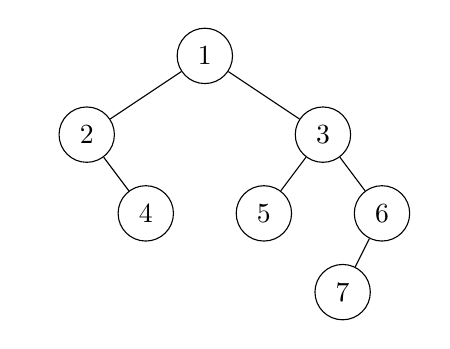
\begin{tikzpicture}[
  every node/.style = {minimum width = 2em, draw, circle},
  level/.style = {level distance=10mm,sibling distance = 30mm/#1}
  ]
  \node {1}
  child {node {2} 
                child {edge from parent[draw = none]}
                child {node {4}}
        }
  child {node {3}
        child {node {5}}
        child {node {6}
                        child {node {7}}
                        child {edge from parent[draw = none]}
               }
        };
\end{tikzpicture}
\end{center}
\caption{Binary tree}
\end{figure}

If we encode number of children information to each node then we get following inorder traversal
\begin{center} 
        [(2,1),(4,0),(1,2),(5,0),(3,2),(7,0),(6,1)]
\end{center}
where first element in tuple is node value and second element is its number of children. But there can be another tree with same inorder traversal and same children count. Following is the another tree with the same inorder traversal and same children count for each node.

\begin{figure}[h!]
\begin{center} 
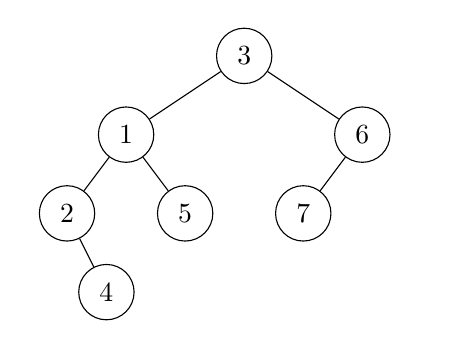
\begin{tikzpicture}[
  every node/.style = {minimum width = 2em, draw, circle},
  level/.style = {level distance=10mm,sibling distance = 30mm/#1}
  ]
  \node {3}
  child {node {1}
        child {node {2}
                child {edge from parent[draw = none]}
                child {node {4}}
        }
        child {node {5}}
        }
  child {node {6} 
                child {node {7}}
                child {edge from parent[draw = none]}
        };
\end{tikzpicture}
\end{center}
\caption{Binary tree with same inorder traversal and number of children}
\end{figure}
So our idea of storing children count of each node with inorder traversal not works as we have counterexample. \\
So we have think about another idea. 
\subsection{Recovery using level}
What if we store level of each node along with the inorder traversal?
Then we can find root of tree easily. Root of tree will be node with level 0. And there will be only one node with level 0. If we split inorder list about root, we also get inorder list for its left subtree and right subtree. The root for each subtree will be the node with minimum level.\\

\nwenddocs{}\nwbegincode{2}\sublabel{NW4896Yo-N7IVZ-1}\nwmargintag{{\nwtagstyle{}\subpageref{NW4896Yo-N7IVZ-1}}}\moddef{inorder~{\nwtagstyle{}\subpageref{NW4896Yo-N7IVZ-1}}}\endmoddef\nwstartdeflinemarkup\nwusesondefline{\\{NW4896Yo-2dJGUc-1}}\nwenddeflinemarkup
local
        fun ino (Empty, Llist, Level) = Llist
                | ino (Node (N, LST, RST), Llist, Level) =
                        let val Mlist = ino (RST, Llist, Level+1)
                                val Nlist = ino (LST, (N,Level)::Mlist, Level+1)
                        in Nlist
                        end
in
        fun inorder T = ino (T, [],0)
end
\nwused{\\{NW4896Yo-2dJGUc-1}}\nwendcode{}\nwbegindocs{3}\nwdocspar

The above inorder function do inorder traversal of binary tree. While doing inorder traversal it also store level of node in tuple. It returns the list of tuples, where each tuple is made of node value and node level. \\
When we do inorder on example tree we get the following inorder traversal
\begin{center}
[(2,1),(4,2),(1,0),(5,2),(3,1),(7,3),(6,2)]
\end{center}
Here we can see that there is only one node with level 0 which has node value 1. So it must be root of tree and all left side of it is inorder traversal of its left subtree and all right side of it is inorder traversal of right subtree. \\
So here is the function of finding root of any subtree. \\

\nwenddocs{}\nwbegincode{4}\sublabel{NW4896Yo-yA1Ck-1}\nwmargintag{{\nwtagstyle{}\subpageref{NW4896Yo-yA1Ck-1}}}\moddef{getRoot~{\nwtagstyle{}\subpageref{NW4896Yo-yA1Ck-1}}}\endmoddef\nwstartdeflinemarkup\nwusesondefline{\\{NW4896Yo-2dJGUc-1}}\nwenddeflinemarkup
fun getRoot [] = NONE
        |  getRoot(List) = 
                let
                        fun getMin(List: ('a * int) list) = 
                                if null (tl List) then (hd List)
                                else
                                        let
                                                val tl_ans = getMin(tl List)
                                        in
                                                if #2 (hd List) < #2 (tl_ans) then (hd List)
                                                else tl_ans
                                        end
                in
                        SOME (getMin(List))
                end
\nwused{\\{NW4896Yo-2dJGUc-1}}\nwendcode{}\nwbegindocs{5}\nwdocspar

Once we found the root, we need to split the list around root to get the inorder traversal of left subtree and right subtree.\\

\nwenddocs{}\nwbegincode{6}\sublabel{NW4896Yo-qWzDz-1}\nwmargintag{{\nwtagstyle{}\subpageref{NW4896Yo-qWzDz-1}}}\moddef{split~{\nwtagstyle{}\subpageref{NW4896Yo-qWzDz-1}}}\endmoddef\nwstartdeflinemarkup\nwusesondefline{\\{NW4896Yo-2dJGUc-1}}\nwenddeflinemarkup
fun split(Min: int, L1: ('a * int) list, L2: ('a * int) list) =
        if Min = #2 (hd L2) then (L1, tl L2)
        else
                let
                        val new_l1 = L1@[hd L2]
                        val new_l2 = tl L2
                in
                        split(Min, new_l1, new_l2)
                end
\nwused{\\{NW4896Yo-2dJGUc-1}}\nwendcode{}\nwbegindocs{7}\nwdocspar

Once we split the list we can build the tree recursively.\\
\nwenddocs{}\nwbegincode{8}\sublabel{NW4896Yo-D88LJ-1}\nwmargintag{{\nwtagstyle{}\subpageref{NW4896Yo-D88LJ-1}}}\moddef{inorderInverse~{\nwtagstyle{}\subpageref{NW4896Yo-D88LJ-1}}}\endmoddef\nwstartdeflinemarkup\nwusesondefline{\\{NW4896Yo-2dJGUc-1}}\nwenddeflinemarkup
fun inorderInverse [] = Empty
        |       inorderInverse List = 
                let
                        val root = valOf(getRoot(List))
                        val rootVal = #1 root
                        val rootLevel = #2 root
                        val (LSTList, RSTList) = split(rootLevel, [], List)
                        val (LST, RST) = (inorderInverse(LSTList), inorderInverse(RSTList))
                in
                        Node(rootVal, LST, RST )
                end
\nwused{\\{NW4896Yo-2dJGUc-1}}\nwendcode{}\nwbegindocs{9}\nwdocspar
\subsection{Complexity}
In the above method we store node level along with the node value. So the our algorithm makes the two times size of inorder traversal list compared to normal inorder traversal.\\
\subsubsection{Comparison with leaf information storing}
If binary tree have N nodes then it have total floor \( \frac{N+1}{2} \) leaf node. So the leaf node information method will take at least 2*\( \frac{N+1}{2} \) = N+1 extra information to store along with node information. One extra information will also have to store for degree-1 node. So we were storing 2 extra information for each leaf node and 1 extra information for each degree-1 node\\
Our algorithm of storing level for each node only takes N extra information in all cases.\\
So our algorithm for storing extra information along with traversal take less number of information but important information.

\section{Making Module}
Now we will make module\\
Datatype representation of binary tree\\
\nwenddocs{}\nwbegincode{10}\sublabel{NW4896Yo-3FQtIp-1}\nwmargintag{{\nwtagstyle{}\subpageref{NW4896Yo-3FQtIp-1}}}\moddef{datatype~{\nwtagstyle{}\subpageref{NW4896Yo-3FQtIp-1}}}\endmoddef\nwstartdeflinemarkup\nwusesondefline{\\{NW4896Yo-GBdPh-1}}\nwenddeflinemarkup
datatype 'a bintree =Empty |
        Node of 'a * 'a bintree * 'a bintree
\nwused{\\{NW4896Yo-GBdPh-1}}\nwendcode{}\nwbegindocs{11}\nwdocspar

Signature of binary tree\\
\nwenddocs{}\nwbegincode{12}\sublabel{NW4896Yo-1h1obp-1}\nwmargintag{{\nwtagstyle{}\subpageref{NW4896Yo-1h1obp-1}}}\moddef{signature~{\nwtagstyle{}\subpageref{NW4896Yo-1h1obp-1}}}\endmoddef\nwstartdeflinemarkup\nwusesondefline{\\{NW4896Yo-GBdPh-1}}\nwenddeflinemarkup
signature BINTREE =
        sig
                
                val root : 'a bintree -> 'a
                val leftSubtree : 'a bintree -> 'a bintree
                val rightSubtree: 'a bintree -> 'a bintree
                val height : 'a bintree -> int
                val size : 'a bintree -> int
                val isLeaf : 'a bintree -> bool
                val inorder : 'a bintree -> ('a *int) list
                val getRoot : ('a * int) list -> ('a * int) option
                val split : int * ('a * int) list * ('a * int) list -> ('a * int) list * ('a * int) list
                val inorderInverse: ('a * int) list -> 'a bintree
        end (* sig *)
\nwused{\\{NW4896Yo-GBdPh-1}}\nwendcode{}\nwbegindocs{13}\nwdocspar

Now we will define basic binary tree functions\\
\nwenddocs{}\nwbegincode{14}\sublabel{NW4896Yo-1EKRTS-1}\nwmargintag{{\nwtagstyle{}\subpageref{NW4896Yo-1EKRTS-1}}}\moddef{emptyexcetion~{\nwtagstyle{}\subpageref{NW4896Yo-1EKRTS-1}}}\endmoddef\nwstartdeflinemarkup\nwusesondefline{\\{NW4896Yo-3lRlgj-1}}\nwenddeflinemarkup
exception Empty_bintree;
\nwused{\\{NW4896Yo-3lRlgj-1}}\nwendcode{}\nwbegindocs{15}\nwdocspar
\nwenddocs{}\nwbegincode{16}\sublabel{NW4896Yo-M1ktB-1}\nwmargintag{{\nwtagstyle{}\subpageref{NW4896Yo-M1ktB-1}}}\moddef{root~{\nwtagstyle{}\subpageref{NW4896Yo-M1ktB-1}}}\endmoddef\nwstartdeflinemarkup\nwusesondefline{\\{NW4896Yo-3lRlgj-1}}\nwenddeflinemarkup
fun root Empty = raise Empty_bintree
        | root (Node (x, _, _)) = x;
\nwused{\\{NW4896Yo-3lRlgj-1}}\nwendcode{}\nwbegindocs{17}\nwdocspar
\nwenddocs{}\nwbegincode{18}\sublabel{NW4896Yo-1t8HkM-1}\nwmargintag{{\nwtagstyle{}\subpageref{NW4896Yo-1t8HkM-1}}}\moddef{leftsubtree~{\nwtagstyle{}\subpageref{NW4896Yo-1t8HkM-1}}}\endmoddef\nwstartdeflinemarkup\nwusesondefline{\\{NW4896Yo-3lRlgj-1}}\nwenddeflinemarkup
fun leftSubtree Empty = raise Empty_bintree
        | leftSubtree (Node (_, LST, _)) = LST;
\nwused{\\{NW4896Yo-3lRlgj-1}}\nwendcode{}\nwbegindocs{19}\nwdocspar
\nwenddocs{}\nwbegincode{20}\sublabel{NW4896Yo-mvyXW-1}\nwmargintag{{\nwtagstyle{}\subpageref{NW4896Yo-mvyXW-1}}}\moddef{rightsubtree~{\nwtagstyle{}\subpageref{NW4896Yo-mvyXW-1}}}\endmoddef\nwstartdeflinemarkup\nwusesondefline{\\{NW4896Yo-3lRlgj-1}}\nwenddeflinemarkup
fun rightSubtree Empty = raise Empty_bintree
        | rightSubtree (Node (_, _, RST)) = RST;
\nwused{\\{NW4896Yo-3lRlgj-1}}\nwendcode{}\nwbegindocs{21}\nwdocspar
\nwenddocs{}\nwbegincode{22}\sublabel{NW4896Yo-13AddF-1}\nwmargintag{{\nwtagstyle{}\subpageref{NW4896Yo-13AddF-1}}}\moddef{height~{\nwtagstyle{}\subpageref{NW4896Yo-13AddF-1}}}\endmoddef\nwstartdeflinemarkup\nwusesondefline{\\{NW4896Yo-3lRlgj-1}}\nwenddeflinemarkup
fun height Empty = 0
        | height (Node (_, left, right)) =
                let
                        val lh = height left
                        val rh = height right
                in 1 + Int.max(lh, rh)
                end;
\nwused{\\{NW4896Yo-3lRlgj-1}}\nwendcode{}\nwbegindocs{23}\nwdocspar
\nwenddocs{}\nwbegincode{24}\sublabel{NW4896Yo-4Hcf9c-1}\nwmargintag{{\nwtagstyle{}\subpageref{NW4896Yo-4Hcf9c-1}}}\moddef{size~{\nwtagstyle{}\subpageref{NW4896Yo-4Hcf9c-1}}}\endmoddef\nwstartdeflinemarkup\nwusesondefline{\\{NW4896Yo-3lRlgj-1}}\nwenddeflinemarkup
fun size Empty = 0
        | size (Node (_, left, right)) =
                let
                        val ls = size left
                        val rs = size right
                in 1 + ls + rs
                end;
\nwused{\\{NW4896Yo-3lRlgj-1}}\nwendcode{}\nwbegindocs{25}\nwdocspar
\nwenddocs{}\nwbegincode{26}\sublabel{NW4896Yo-1VK7YD-1}\nwmargintag{{\nwtagstyle{}\subpageref{NW4896Yo-1VK7YD-1}}}\moddef{isleaf~{\nwtagstyle{}\subpageref{NW4896Yo-1VK7YD-1}}}\endmoddef\nwstartdeflinemarkup\nwusesondefline{\\{NW4896Yo-3lRlgj-1}}\nwenddeflinemarkup
fun isLeaf Empty = false
        | isLeaf (Node (_, Empty, Empty)) = true
        | isLeaf _ = false;
\nwused{\\{NW4896Yo-3lRlgj-1}}\nwendcode{}\nwbegindocs{27}\nwdocspar
So the basic binary tree functions will look like this \\

\nwenddocs{}\nwbegincode{28}\sublabel{NW4896Yo-3lRlgj-1}\nwmargintag{{\nwtagstyle{}\subpageref{NW4896Yo-3lRlgj-1}}}\moddef{basicbintree~{\nwtagstyle{}\subpageref{NW4896Yo-3lRlgj-1}}}\endmoddef\nwstartdeflinemarkup\nwusesondefline{\\{NW4896Yo-2dJGUc-1}}\nwenddeflinemarkup
\LA{}emptyexcetion~{\nwtagstyle{}\subpageref{NW4896Yo-1EKRTS-1}}\RA{}
\LA{}root~{\nwtagstyle{}\subpageref{NW4896Yo-M1ktB-1}}\RA{}
\LA{}leftsubtree~{\nwtagstyle{}\subpageref{NW4896Yo-1t8HkM-1}}\RA{}
\LA{}rightsubtree~{\nwtagstyle{}\subpageref{NW4896Yo-mvyXW-1}}\RA{}
\LA{}height~{\nwtagstyle{}\subpageref{NW4896Yo-13AddF-1}}\RA{}
\LA{}size~{\nwtagstyle{}\subpageref{NW4896Yo-4Hcf9c-1}}\RA{}
\LA{}isleaf~{\nwtagstyle{}\subpageref{NW4896Yo-1VK7YD-1}}\RA{}
\nwused{\\{NW4896Yo-2dJGUc-1}}\nwendcode{}\nwbegindocs{29}\nwdocspar

Now structure of module will look like this\\
\nwenddocs{}\nwbegincode{30}\sublabel{NW4896Yo-2dJGUc-1}\nwmargintag{{\nwtagstyle{}\subpageref{NW4896Yo-2dJGUc-1}}}\moddef{structure~{\nwtagstyle{}\subpageref{NW4896Yo-2dJGUc-1}}}\endmoddef\nwstartdeflinemarkup\nwusesondefline{\\{NW4896Yo-GBdPh-1}}\nwenddeflinemarkup
structure Bintree : BINTREE =
   struct
   \LA{}basicbintree~{\nwtagstyle{}\subpageref{NW4896Yo-3lRlgj-1}}\RA{}
   \LA{}inorder~{\nwtagstyle{}\subpageref{NW4896Yo-N7IVZ-1}}\RA{}
   \LA{}getRoot~{\nwtagstyle{}\subpageref{NW4896Yo-yA1Ck-1}}\RA{}
   \LA{}split~{\nwtagstyle{}\subpageref{NW4896Yo-qWzDz-1}}\RA{}
   \LA{}inorderInverse~{\nwtagstyle{}\subpageref{NW4896Yo-D88LJ-1}}\RA{}
   end
\nwused{\\{NW4896Yo-GBdPh-1}}\nwendcode{}\nwbegindocs{31}\nwdocspar

Now complete module will look like this\\
\nwenddocs{}\nwbegincode{32}\sublabel{NW4896Yo-GBdPh-1}\nwmargintag{{\nwtagstyle{}\subpageref{NW4896Yo-GBdPh-1}}}\moddef{2019MCS2565-module-complete.sml~{\nwtagstyle{}\subpageref{NW4896Yo-GBdPh-1}}}\endmoddef\nwstartdeflinemarkup\nwenddeflinemarkup
\LA{}datatype~{\nwtagstyle{}\subpageref{NW4896Yo-3FQtIp-1}}\RA{}
\LA{}signature~{\nwtagstyle{}\subpageref{NW4896Yo-1h1obp-1}}\RA{}
\LA{}structure~{\nwtagstyle{}\subpageref{NW4896Yo-2dJGUc-1}}\RA{}
\nwnotused{2019MCS2565-module-complete.sml}\nwendcode{}\nwbegindocs{33}\nwdocspar

\section{Test cases}
Test cases\\
\nwenddocs{}\nwbegincode{34}\sublabel{NW4896Yo-3kROYe-1}\nwmargintag{{\nwtagstyle{}\subpageref{NW4896Yo-3kROYe-1}}}\moddef{use~{\nwtagstyle{}\subpageref{NW4896Yo-3kROYe-1}}}\endmoddef\nwstartdeflinemarkup\nwusesondefline{\\{NW4896Yo-2Ag6yI-1}\\{NW4896Yo-1VsZET-1}\\{NW4896Yo-1QUbrk-1}\\{NW4896Yo-DmyLe-1}}\nwenddeflinemarkup
use "2019MCS2565-module-complete.sml";
\nwused{\\{NW4896Yo-2Ag6yI-1}\\{NW4896Yo-1VsZET-1}\\{NW4896Yo-1QUbrk-1}\\{NW4896Yo-DmyLe-1}}\nwendcode{}\nwbegindocs{35}\nwdocspar
\nwenddocs{}\nwbegincode{36}\sublabel{NW4896Yo-Joiug-1}\nwmargintag{{\nwtagstyle{}\subpageref{NW4896Yo-Joiug-1}}}\moddef{test~{\nwtagstyle{}\subpageref{NW4896Yo-Joiug-1}}}\endmoddef\nwstartdeflinemarkup\nwusesondefline{\\{NW4896Yo-2Ag6yI-1}\\{NW4896Yo-1VsZET-1}\\{NW4896Yo-1QUbrk-1}\\{NW4896Yo-DmyLe-1}}\nwenddeflinemarkup
val traversal = Bintree.inorder t1;
val tree = Bintree.inorderInverse traversal;
\nwused{\\{NW4896Yo-2Ag6yI-1}\\{NW4896Yo-1VsZET-1}\\{NW4896Yo-1QUbrk-1}\\{NW4896Yo-DmyLe-1}}\nwendcode{}\nwbegindocs{37}\nwdocspar
Test case 1\\
This is test case for skewed tree which has only right child
\nwenddocs{}\nwbegincode{38}\sublabel{NW4896Yo-2Ag6yI-1}\nwmargintag{{\nwtagstyle{}\subpageref{NW4896Yo-2Ag6yI-1}}}\moddef{2019MCS2565-case1-complete.sml~{\nwtagstyle{}\subpageref{NW4896Yo-2Ag6yI-1}}}\endmoddef\nwstartdeflinemarkup\nwenddeflinemarkup
\LA{}use~{\nwtagstyle{}\subpageref{NW4896Yo-3kROYe-1}}\RA{}
val t4 = Node (4, Empty, Empty);
val t3 = Node (3, Empty, t4);
val t2 = Node (2, Empty, t3);
val t1 = Node (1, Empty, t2);
\LA{}test~{\nwtagstyle{}\subpageref{NW4896Yo-Joiug-1}}\RA{}
\nwnotused{2019MCS2565-case1-complete.sml}\nwendcode{}\nwbegindocs{39}\nwdocspar
Test case 2\\
This is test case for example tree given in this document
\nwenddocs{}\nwbegincode{40}\sublabel{NW4896Yo-1VsZET-1}\nwmargintag{{\nwtagstyle{}\subpageref{NW4896Yo-1VsZET-1}}}\moddef{2019MCS2565-case2-complete.sml~{\nwtagstyle{}\subpageref{NW4896Yo-1VsZET-1}}}\endmoddef\nwstartdeflinemarkup\nwenddeflinemarkup
\LA{}use~{\nwtagstyle{}\subpageref{NW4896Yo-3kROYe-1}}\RA{}
val t7 = Node (7, Empty, Empty);
val t6 = Node (6, t7, Empty);
val t5 = Node (5, Empty, Empty);
val t4 = Node (4, Empty, Empty);
val t3 = Node (3, t5, t6);
val t2 = Node (2, Empty, t4);
val t1 = Node (1, t2, t3);
\LA{}test~{\nwtagstyle{}\subpageref{NW4896Yo-Joiug-1}}\RA{}
\nwnotused{2019MCS2565-case2-complete.sml}\nwendcode{}\nwbegindocs{41}\nwdocspar
Test case 3\\
This is test case for skewed tree which has only left child
\nwenddocs{}\nwbegincode{42}\sublabel{NW4896Yo-1QUbrk-1}\nwmargintag{{\nwtagstyle{}\subpageref{NW4896Yo-1QUbrk-1}}}\moddef{2019MCS2565-case3-complete.sml~{\nwtagstyle{}\subpageref{NW4896Yo-1QUbrk-1}}}\endmoddef\nwstartdeflinemarkup\nwenddeflinemarkup
\LA{}use~{\nwtagstyle{}\subpageref{NW4896Yo-3kROYe-1}}\RA{}
val t4 = Node (4, Empty, Empty);
val t3 = Node (3, t4, Empty);
val t2 = Node (2, t3, Empty);
val t1 = Node (1, t2, Empty);
\LA{}test~{\nwtagstyle{}\subpageref{NW4896Yo-Joiug-1}}\RA{}
\nwnotused{2019MCS2565-case3-complete.sml}\nwendcode{}\nwbegindocs{43}\nwdocspar
Test case 4\\
This is test case single node tree
\nwenddocs{}\nwbegincode{44}\sublabel{NW4896Yo-DmyLe-1}\nwmargintag{{\nwtagstyle{}\subpageref{NW4896Yo-DmyLe-1}}}\moddef{2019MCS2565-case4-complete.sml~{\nwtagstyle{}\subpageref{NW4896Yo-DmyLe-1}}}\endmoddef\nwstartdeflinemarkup\nwenddeflinemarkup
\LA{}use~{\nwtagstyle{}\subpageref{NW4896Yo-3kROYe-1}}\RA{}
val t1 = Node (1, Empty, t1);
\LA{}test~{\nwtagstyle{}\subpageref{NW4896Yo-Joiug-1}}\RA{}
\nwnotused{2019MCS2565-case4-complete.sml}\nwendcode{}

\nwixlogsorted{c}{{2019MCS2565-case1-complete.sml}{NW4896Yo-2Ag6yI-1}{\nwixd{NW4896Yo-2Ag6yI-1}}}%
\nwixlogsorted{c}{{2019MCS2565-case2-complete.sml}{NW4896Yo-1VsZET-1}{\nwixd{NW4896Yo-1VsZET-1}}}%
\nwixlogsorted{c}{{2019MCS2565-case3-complete.sml}{NW4896Yo-1QUbrk-1}{\nwixd{NW4896Yo-1QUbrk-1}}}%
\nwixlogsorted{c}{{2019MCS2565-case4-complete.sml}{NW4896Yo-DmyLe-1}{\nwixd{NW4896Yo-DmyLe-1}}}%
\nwixlogsorted{c}{{2019MCS2565-module-complete.sml}{NW4896Yo-GBdPh-1}{\nwixd{NW4896Yo-GBdPh-1}}}%
\nwixlogsorted{c}{{basicbintree}{NW4896Yo-3lRlgj-1}{\nwixd{NW4896Yo-3lRlgj-1}\nwixu{NW4896Yo-2dJGUc-1}}}%
\nwixlogsorted{c}{{datatype}{NW4896Yo-3FQtIp-1}{\nwixd{NW4896Yo-3FQtIp-1}\nwixu{NW4896Yo-GBdPh-1}}}%
\nwixlogsorted{c}{{emptyexcetion}{NW4896Yo-1EKRTS-1}{\nwixd{NW4896Yo-1EKRTS-1}\nwixu{NW4896Yo-3lRlgj-1}}}%
\nwixlogsorted{c}{{getRoot}{NW4896Yo-yA1Ck-1}{\nwixd{NW4896Yo-yA1Ck-1}\nwixu{NW4896Yo-2dJGUc-1}}}%
\nwixlogsorted{c}{{height}{NW4896Yo-13AddF-1}{\nwixd{NW4896Yo-13AddF-1}\nwixu{NW4896Yo-3lRlgj-1}}}%
\nwixlogsorted{c}{{inorder}{NW4896Yo-N7IVZ-1}{\nwixd{NW4896Yo-N7IVZ-1}\nwixu{NW4896Yo-2dJGUc-1}}}%
\nwixlogsorted{c}{{inorderInverse}{NW4896Yo-D88LJ-1}{\nwixd{NW4896Yo-D88LJ-1}\nwixu{NW4896Yo-2dJGUc-1}}}%
\nwixlogsorted{c}{{isleaf}{NW4896Yo-1VK7YD-1}{\nwixd{NW4896Yo-1VK7YD-1}\nwixu{NW4896Yo-3lRlgj-1}}}%
\nwixlogsorted{c}{{leftsubtree}{NW4896Yo-1t8HkM-1}{\nwixd{NW4896Yo-1t8HkM-1}\nwixu{NW4896Yo-3lRlgj-1}}}%
\nwixlogsorted{c}{{rightsubtree}{NW4896Yo-mvyXW-1}{\nwixd{NW4896Yo-mvyXW-1}\nwixu{NW4896Yo-3lRlgj-1}}}%
\nwixlogsorted{c}{{root}{NW4896Yo-M1ktB-1}{\nwixd{NW4896Yo-M1ktB-1}\nwixu{NW4896Yo-3lRlgj-1}}}%
\nwixlogsorted{c}{{signature}{NW4896Yo-1h1obp-1}{\nwixd{NW4896Yo-1h1obp-1}\nwixu{NW4896Yo-GBdPh-1}}}%
\nwixlogsorted{c}{{size}{NW4896Yo-4Hcf9c-1}{\nwixd{NW4896Yo-4Hcf9c-1}\nwixu{NW4896Yo-3lRlgj-1}}}%
\nwixlogsorted{c}{{split}{NW4896Yo-qWzDz-1}{\nwixd{NW4896Yo-qWzDz-1}\nwixu{NW4896Yo-2dJGUc-1}}}%
\nwixlogsorted{c}{{structure}{NW4896Yo-2dJGUc-1}{\nwixd{NW4896Yo-2dJGUc-1}\nwixu{NW4896Yo-GBdPh-1}}}%
\nwixlogsorted{c}{{test}{NW4896Yo-Joiug-1}{\nwixd{NW4896Yo-Joiug-1}\nwixu{NW4896Yo-2Ag6yI-1}\nwixu{NW4896Yo-1VsZET-1}\nwixu{NW4896Yo-1QUbrk-1}\nwixu{NW4896Yo-DmyLe-1}}}%
\nwixlogsorted{c}{{use}{NW4896Yo-3kROYe-1}{\nwixd{NW4896Yo-3kROYe-1}\nwixu{NW4896Yo-2Ag6yI-1}\nwixu{NW4896Yo-1VsZET-1}\nwixu{NW4896Yo-1QUbrk-1}\nwixu{NW4896Yo-DmyLe-1}}}%
\nwbegindocs{45}\nwdocspar
\end{document}
\nwenddocs{}
